\documentclass[tikz,border=7pt]{standalone}
\usepackage{amsmath,amssymb}
\usepackage[scaled]{helvet}
\renewcommand{\familydefault}{\sfdefault}
\usetikzlibrary{arrows.meta,backgrounds,calc,fit,positioning,shapes.geometric}
\definecolor{bpink}{HTML}{172033}
\definecolor{bpblue}{HTML}{2A78D6}
\definecolor{bporange}{HTML}{E56A32}
\definecolor{bpgreen}{HTML}{168A65}
\definecolor{bppurple}{HTML}{7A5CC7}
\definecolor{bpred}{HTML}{C94A4A}
\definecolor{bpmuted}{HTML}{667085}
\definecolor{bpgrid}{HTML}{D8DEE8}
\definecolor{bpsurface}{HTML}{F8FAFC}
\tikzset{
  var/.style={circle,draw=bpblue,fill=bpblue!10,line width=.9pt,minimum size=8mm,font=\small\bfseries,text=bpink},
  factor/.style={rectangle,rounded corners=1.5pt,draw=bporange,fill=bporange!14,line width=.9pt,minimum size=6.8mm,font=\small\bfseries,text=bpink},
  constraint/.style={rectangle,rounded corners=1.5pt,draw=bpred,fill=bpred!12,line width=.9pt,minimum size=6.8mm,font=\small\bfseries,text=bpink},
  edge/.style={draw=bpmuted!75,line width=.9pt},
  msgvf/.style={-{Latex[length=2.2mm]},draw=bpblue,line width=1.35pt},
  msgfv/.style={-{Latex[length=2.2mm]},draw=bporange,line width=1.35pt},
  label/.style={font=\scriptsize,text=bpmuted,align=center},
  title/.style={font=\bfseries\large,text=bpink},
  card/.style={draw=bpgrid,fill=bpsurface,rounded corners=7pt,line width=.7pt},
}

\begin{document}
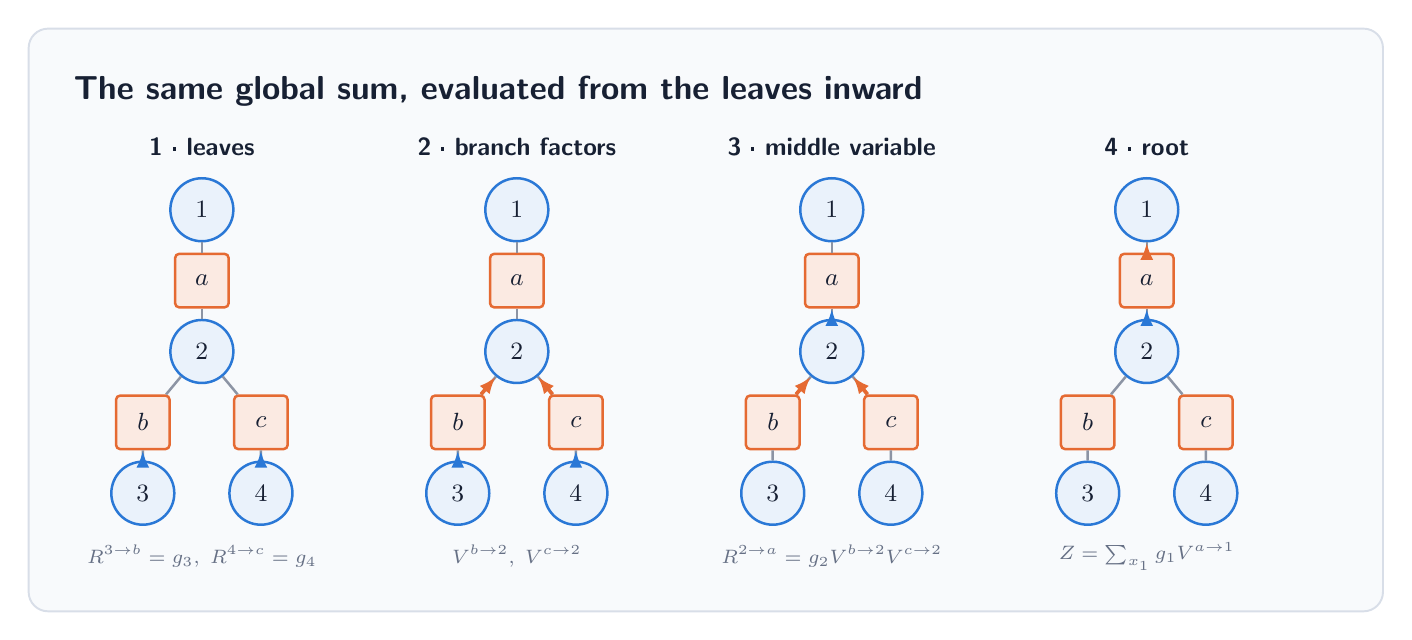
\begin{tikzpicture}[font=\sffamily]
  \node[card,minimum width=17.2cm,minimum height=7.4cm] at (7.8,2.25) {};
  \node[title,anchor=west] at (-.35,5.15) {The same global sum, evaluated from the leaves inward};
  \foreach \x/\lab in {0/{1 · leaves},4/{2 · branch factors},8/{3 · middle variable},12/{4 · root}} {
    \node[text=bpink,font=\small\bfseries] at (\x+1.4,4.45) {\lab};
  }
  \foreach \shift in {0,4,8,12} {
    \node[var] (r\shift) at (\shift+1.4,3.65) {$1$};
    \node[factor] (a\shift) at (\shift+1.4,2.75) {$a$};
    \node[var] (m\shift) at (\shift+1.4,1.85) {$2$};
    \node[factor] (b\shift) at (\shift+.65,.95) {$b$};
    \node[factor] (c\shift) at (\shift+2.15,.95) {$c$};
    \node[var] (l\shift) at (\shift+.65,.05) {$3$};
    \node[var] (q\shift) at (\shift+2.15,.05) {$4$};
    \draw[edge] (r\shift)--(a\shift)--(m\shift);
    \draw[edge] (m\shift)--(b\shift)--(l\shift);
    \draw[edge] (m\shift)--(c\shift)--(q\shift);
  }
  \draw[msgvf] (l0)--(b0); \draw[msgvf] (q0)--(c0);
  \draw[msgvf] (l4)--(b4); \draw[msgvf] (q4)--(c4); \draw[msgfv] (b4)--(m4); \draw[msgfv] (c4)--(m4);
  \draw[msgfv] (b8)--(m8); \draw[msgfv] (c8)--(m8); \draw[msgvf] (m8)--(a8);
  \draw[msgvf] (m12)--(a12); \draw[msgfv] (a12)--(r12);
  \node[label] at (1.4,-.75) {$R^{3\to b}=g_3,\;R^{4\to c}=g_4$};
  \node[label] at (5.4,-.75) {$V^{b\to2},\;V^{c\to2}$};
  \node[label] at (9.4,-.75) {$R^{2\to a}=g_2V^{b\to2}V^{c\to2}$};
  \node[label] at (13.4,-.75) {$Z=\sum_{x_1}g_1V^{a\to1}$};
\end{tikzpicture}
\end{document}
